%% 
%% Copyright 2019-2020 Elsevier Ltd
%% 
%% This file is part of the 'CAS Bundle'.
%% --------------------------------------
%% 
%% It may be distributed under the conditions of the LaTeX Project Public
%% License, either version 1.2 of this license or (at your option) any
%% later version.  The latest version of this license is in
%%    http://www.latex-project.org/lppl.txt
%% and version 1.2 or later is part of all distributions of LaTeX
%% version 1999/12/01 or later.
%% 
%% The list of all files belonging to the 'CAS Bundle' is
%% given in the file `manifest.txt'.
%% 
%% Template article for cas-sc documentclass for 
%% single column output.

%\documentclass[a4paper,fleqn,longmktitle]{cas-sc}
\documentclass[a4paper,fleqn]{cas-sc}

%\usepackage[numbers]{natbib}
%\usepackage[authoryear]{natbib}
\usepackage[square,numbers]{natbib}

\usepackage{url}
%\usepackage{cite}
\usepackage{amsmath,amssymb,amsfonts}
\usepackage{algorithmic}
\usepackage{graphicx}
\usepackage{textcomp}
\usepackage{empheq} 
\usepackage{xcolor}
\newcommand*{\MyDef}{\mathrm{def}}
\newcommand*{\eqdefU}{\ensuremath{\mathop{\overset{\MyDef}{=}}}}
\newcommand*{\eqde}{\ensuremath{\mathop{\overset{\MyDef}{=}}}}
\newcommand\Z{\mathbb{Z}}
\newcommand\N{\mathbb{N}}
\newcommand\R{\mathbb{R}}
\newcommand\calF{\mathcal{F}}
\newcommand\calW{\mathcal{W}}
\newcommand\calS{\mathcal{S}}
\newcommand\esp[1]{{\mathchoice{\besp{#1}}{\sesp{#1}}{\sesp{#1}}{\sesp{#1}}}}
\newcommand\besp[1]{\mathbb{E}\left[#1\right]}
\newcommand\sesp[1]{\mathbb{E}[#1]}
\newcommand\Proba[1]{{\mathchoice{\bProba{#1}}{\sProba{#1}}{\sProba{#1}}{\sProba{#1}}}} 
\newcommand\bProba[1]{\mathbb{P}\left[#1\right]}
\newcommand\sProba[1]{\mathbb{P}[#1]}
\newcommand\norm[1]{{\mathchoice{\bnorm{#1}}{\snorm{#1}}{\snorm{#1}}{\snorm{#1}}}}
\newcommand\bnorm[1]{\left\|#1\right\|}
\newcommand\snorm[1]{\|#1\|}
\newcommand\red[1]{{\color{red}#1}}
\usepackage{enumitem}
%\usepackage{hyperref}
%\definecolor{darkblue}{rgb}{0 0 .6}
%\hypersetup{%
%  colorlinks=true, linktocpage=true, pdfstartpage=3, pdfstartview=FitV,%
%  linkcolor=darkblue,citecolor=darkblue,urlcolor=darkblue
%}
 \newtheorem{theorem}{Theorem}
 \newtheorem{lemma}[theorem]{Lemma}
 \newdefinition{rmk}{Remark}
 \newproof{proof}{Proof}
 \newproof{pf}{Proof}
 \newproof{pot}{Proof of Theorem \ref{thm2}}
\renewlist{cases}{enumerate}{10}
\setlist[cases]{label=\textbf{Case \arabic*}, itemindent=0pt,leftmargin=35pt,  listparindent=1.5 em}

\newcommand\nbworkrequest{\#\text{\{Work Requests\}}}

%%%Author macros
\def\tsc#1{\csdef{#1}{\textsc{\lowercase{#1}}\xspace}}
\tsc{WGM}
\tsc{QE}
\tsc{EP}
\tsc{PMS}
\tsc{BEC}
\tsc{DE}
%%%

\begin{document}
\let\WriteBookmarks\relax
\def\floatpagepagefraction{1}
\def\textpagefraction{.001}
\shorttitle{Analysis of Work Stealing with latency}
\shortauthors{Nicolas Gast et~al.}
%\begin{frontmatter}

\title [mode = title]{Analysis of Work Stealing with latency}                      
%\tnotemark[1,2]


\author[1]{Nicolas Gast}
\author[1,2]{Mohammed Khatiri}
\author[1]{Denis Trystram}
\author[1]{Fr\'ed\'eric Wagner}

                                                
\address[1]{Univ. Grenoble Alpes, Inria, CNRS, Grenoble INP, LIG, 38000 Grenoble, France}
\address[2]{University Mohammed First, Faculty of Sciences, LaRI, 60000, Oujda, Morocco}
\address[]{Email: firstname.lastname@inria.fr} 


%\affil[ ]{Email: firstname.lastname@inria.fr}  


\begin{abstract}
 We study the impact of communication latency on the
  classical \emph{Work Stealing} load balancing algorithm.  Our paper
  extends the reference model in which we introduce a latency
  parameter. By using a theoretical analysis and simulation, we study
  the overall impact of this latency on the Makespan (maximum
  completion time). We derive a new expression of the expected
  running time of a \textit{bag of independent tasks} scheduled by Work Stealing.
  This expression enables us to predict under which conditions a given run
  will yield acceptable performance. For instance, we can easily
  calibrate the maximal number of processors to use for a given
  work/platform combination.  All our results are validated through
  simulation on a wide range of parameters.
\end{abstract}


%\begin{graphicalabstract}
%\includegraphics{figs/grabs.pdf}
%\end{graphicalabstract}
%
%\begin{highlights}
%\item Research highlights item 1
%\item Research highlights item 2
%\item Research highlights item 3
%\end{highlights}

\begin{keywords}
Work Stealing, Latency, Makespan Analysis
\end{keywords}


\maketitle

% !TEX root = ./main.tex
\section{Introduction}
\label{sec:intro}

Work stealing (WS) is a distributed on-line scheduling algorithm
proposed for shared-memory multi-cores~\cite{Arora2001}. With work
stealing, each processor maintains a local list of tasks to be
executed. When a processor has executed all its local work, it probes
others by sending work requests to randomly chosen processors. We say
that this processor attempts to ``\emph{steal}'' work from others.
Despite its apparent simplicity, work stealing has been proven to be
very effective for scheduling tasks in shared-memory homogeneous
architectures~\cite{Blumofe1999}. Today, the research on WS is driven
by the question on how to extend the analysis for the characteristics
of new computing platforms (distributed memory, large scale,
heterogeneity).  Notice that beside its theoretical interest, WS has
been implemented successfully in several languages and parallel
libraries including Cilk~\cite{Leiserson1998,Leiserson2009}, TBB
(Threading Building Blocks)~\cite{Robison2008}, the PGAS
language~\cite{Dinan2009,Seung-Jai2011} and the KAAPI run-time
system~\cite{Kaapi2007}.

% The performance of a scheduling algorithm is defined by the
% \textit{Makespan}, defined as the maximum completion time of the
% parallel application.

In this paper, we study the performance of WS in a distributed-memory
context.
Such an architecture consists of independent processing elements with
private local memories linked by an interconnection
network. Communication latency is crucial and highly influences the
performance of the applications~\cite{MCMCA}. 
% However, there are only few works dealing with optimized allocation strategies and the relationships with the allocation and scheduling process is most often ignored.
The impact of scheduling is important since the whole execution can be
highly affected by a large communication latency of interconnection
networks~\cite{MultiCoreClusterArchitectur2015}.


%Principle of WS
% WS is an efficient scheduling mechanism targeting medium range parallelism of multi-cores for fine-grain tasks.
% Its principle is briefly recalled as follows:
% each processor manages its own (local) list of tasks.
% When a processor becomes idle, it randomly chooses another processor and steals some work (if possible).
% Its analysis is probabilistic since the algorithm itself is randomized.





\paragraph{Contributions}%  We present a theoretical analysis for an
% upper bound of the expected makespan and we run a complementary series
% of simulations in order to assess how this new bound behaves in
% practice depending on the value of the latency.
In this work, we study how communication latency impacts work
stealing.  Our work has four main contributions. First, we create a
new realistic scheduling model for distributed-memory clusters of $p$
identical processors including latency (denoted by $\lambda$).  Second,
we provide an upper bound of the expected makespan to execute a bag of
$\calW$ independent unitary tasks by $p$ processors.  This bound is
the sum of two terms. The first is the usual lower bound on the best
possible load-balancing~$\frac{\mathcal{W}}{p}$; The second term is
proportional to $\lambda\log(\frac{\mathcal{W}}{\lambda})$.
%The additional term depends on the dependence model. In the case of independent tasks, this additional term is
%$16\lambda\log_2(\frac{\mathcal{W}}{\lambda})$.
%In the case of DAG, this term is proportional to the critical path.
Third, we develop a lightweight Python simulator for running adequate
experiments. Our simulator is developed to be flexible enough to
simulate different topologies and applications with different variants
of Work Stealing algorithms.
%This simulator uses the Work Stealing algorithm to schedule an amount of
%work W in a distributed platform composed of p
%identical processors. 
The code is available on GitHub (\url{https://wssimulator.github.io})
along logs of presented experiments. The simulator is
generic enough to be used in different contexts of online
scheduling and interfaces with standard trace analysis
tools
Using this simulator,
we provide simulation results that challenges this bound.
%in the case of indepedent tasks.
These experiments show that the second additional term has indeed the
form $c\lambda\log_2(\frac{\mathcal{W}}{\lambda})$, with
$c\approx3.8$. Note that our theoretical upper bound shows that
$c\le16.12$.  Finally, we show that our methodology can be easily
extended to the case of tasks with precedence. We provide an upper
bound of the expected makespan in this case. This bound is also
composed of two terms. The first is the usual lower bound
$\frac{\mathcal{W}}{p}$ and the second additional term is proportional to the
critical path ($6\lambda D$)

Our analyses are based on the use of adequate potential
functions. While the overall approach is similar to existing work, and in
particular \cite{Denis2013}, there are two technical difficulties that
had to be lifted.  First, a natural extension of the potential
functions used in \cite{Denis2013} does not work as one needs to
account for the work in transit. Second, we do not assume that task
execution and steal requests are synchronized.  This leads to consider
time steps of duration equal to the communication latency.

The rest of the paper is organized as follows.  We review the related works
in Section~\ref{sec:relatedworks}. We present the independent task
model in Section~\ref{sec:wsmechanisms}. We derive our main technical
result in Section~\ref{sec:analysis_indep} in which we obtain a bound
on the makespan. We introduce our work stealing simulator in
Section~\ref{sec:experiemnts} that we use to study the limits of our
analysis. We show how to extend our analysis to tasks with precedence
in Section~\ref{sec:dagOfPrecedence} and conclude in
Section~\ref{sec:conclusion}.  Last, Appendix~\ref{sec:proofs} contains
some technical proofs. 

\section{Related Work}
\label{sec:relatedworks}

Let us first introduce the problem of scheduling:
It is the process which aims at determining where and when to execute the tasks of a target parallel application.
The applications are represented as directed acyclic graphs where the vertices are the basic operations and the arcs are the dependencies between the tasks~\cite{CosnardTrystram92}.
Scheduling is a crucial problem which has been extensively studied under many variants for the successive generations of parallel and distributed systems.
The most commonly studied objective is to minimize the makespan (denoted by $C_{\max}$) and the underlying context is usually to consider centralized algorithms.
This assumption is not always realistic, especially if we consider distributed memory allocations and an on-line setting.
% (called \emph{Makespan} and denoted by $C_{\max}$)


Work Stealing (WS) is a distributed version of scheduling that received sustained attention over the last twenty years. 
It has been studied originally by Blumofe and Leiserson
in~\cite{Blumofe1999}.  They showed that the expected Makespan of a
series-parallel precedence graph with $\mathcal{W}$ unit tasks on $p$
processors is bounded by
$E(C_{\max}) \leq \frac{\mathcal{W}}{p}+\mathcal{O}(D)$ where $D$ is
the length of the critical path of the graph (its depth).  This
analysis has been improved in Arora \textit{et al.}~\cite{Arora2001}
using potential functions.  The case of varying processor speeds has
been studied by Bender and Rabin in~\cite{Bender2002} where the
authors introduced a new policy called \textit{high utilization
  scheduler} that extends the homogeneous case.  The specific case of
tree-shaped computations with a more accurate model has been studied
in~\cite{Sanders1999}.  However, in all these previous analyses, the
precedence graph is constrained to have only one source and an
out-degree of at most 2 which does not easily model the basic case of
independent tasks.  Simulating independent tasks with a binary
precedences tree gives a bound of
$\frac{\mathcal{W}}{p}+\mathcal{O}(\log_2 (\mathcal{W}))$ since a
complete binary tree of $\mathcal{W}$ vertices has a depth
$D \leq \log_2 (\mathcal{W})$.  However, with this approach, the
structure of the binary tree dictates which tasks are stolen. More
recently, in \cite{Denis2013}, Tchiboukjian \textit{et al.} provided
the best bound known at this time:
$\frac{\mathcal{W}}{p}+c.(\log_2 \mathcal{W})+\Theta(1)$ where
$c\approx3.24$.

Acar \emph{et al.}~\cite{Acar2000,Acar2002} studied data locality of
WS on shared-memory and focus on cache misses.  The underlying model
assumes that the execution time takes $m$ time units if the
instruction incurs a cache miss and $1$ unit otherwise.  A steal
attempt takes at least $s$ and at most $ks$ steps to complete ($k\ge1$
multiple steal attempts before succeeding).  When a steal succeeds,
the thief starts working on the stolen task at the next step.  This
model is similar to the classical WS model without communication since
the thief does not wait several time steps to receive the stolen task.

In complement,~\cite{Gast2010,Mitzenmache1998} provided a theoretical
analysis based on a Markovian model using mean field theory. They
targeted the expectation of the average response time and showed that
the system converges to a deterministic Ordinary Differential
Equation.  Note that there exist other results that study the steady
state performance of WS when the work generation is random including
Berenbrink \textit{et al.}~\cite{Berenbrink2003}, Lueling and
Monien~\cite{Lueling1993} and Rudolph \textit{et al.}~\cite{Rudolph1991}.  
%\bigskip

%extension vers les comm


In all these previous theoretical results, communications are not directly addressed
(or at least they are taken implicitly into account by the underlying model).
Most studies on WS largely focused on shared memory systems and 
its performance on modern platforms (distributed-memory systems, hierarchical platform, clusters with explicit communication cost) is not really well understood. 
The difficulty lies in the problems of communication which become more crucial in modern platforms~\cite{Arafat2016}.
Let us briefly review the most relevant works dealing with WS with communications.

%Furthermore, the communication issues become even more crucial in heterogeneous distributed systems
%In shared-memory systems the thieves constantly attempt to asynchronously steal work from randomly chosen victims
%until they find work. In distributed-memory systems, it is much harder since the thieves cannot autonomously steal
%work from a victim without disrupting its execution~\cite{Saraswat2011}.
%WS algorithms are based on shared memory multicore chips, 
Dinan \textit{et al.}~\cite{Dinan2009} implemented WS on large-scale clusters,
and proposed to split each tasks queues into a part accessed asynchronously by local processes 
and a shared portion synchronized by a lock which can be access by any remote processes in order to reduce contention.
%In-place task creation which optimize critical operations. 
%Multi-core processor based on NUMA (non-uniform memory access) architecture is the mainstream today and such new platforms include accelerators as GPGPU~\cite{Yang2017}. 
The authors propose an efficient task management mechanism which is to divide the application into a large
number of fine grained tasks which generate a large amount of small communications between the CPU and the GPGPU accelerators.
However, these data transmissions are very slow.
They consider that the transmission time of small data and large data is the same. 


Besides the large literature on theoretical works, there exist more practical studies implementing WS libraries where some attempts were provided for taking into account communications:
%practical
SLAW is a task-based library introduced in~\cite{Gue2010}, combining work-first
and help-first scheduling policies focused on locality awareness 
in PGAS (Partitioned Global Address Space) languages like UPC (Unified Parallel C). 
It has been extended in HotSLAW, which provides a high level API that abstracts concurrent task management~\cite{Seung-Jai2011}.
\cite{Shigang2013} proposes an asynchronous WS (AsynchWS) strategy which exploits opportunities to overlap communication with
local tasks allowing to hide high communication overheads in distributed memory systems. 
The principle is based on a hierarchical victim selection, also based on PGAS.
Perarnau and Sato presented in~\cite{swann2014} an experimental evaluation of WS on the scale of ten thousands compute nodes where the communication depends on the distance between the nodes.
They investigated in detail the impact of the communication on the performance. In particular, the physical distance between remote nodes is taken into account.
Mullet \textit{et al.} studied in~\cite{Muller2106} 
Latency-Hiding, a new WS algorithm that hides the overhead
caused by some operations, such as waiting for a request from a client or waiting
for a response from a remote machine.
The authors refer to this delay as \emph{latency} which is slightly
different that the more general concept we consider in our paper. 
Agrawal \textit{et al.} proposed in~\cite{Agrawal} an analysis showing the optimality for task graphs with bounded degrees
and they developed a library in Cilk++ called \textit{Nabbit} for executing tasks
with arbitrary dependencies, with reasonable block sizes.

%\bigskip

%\cite{Jixiang Yang xx }

%Traditional work stealing strategy mainly verifies its performance by simulation data
%or individual applications and concludes corresponding results. Parallel
%computing becomes popular in multi-core era, and it is not persuasive to verify
%scheduling performance just by selecting experimental data for individual applications,
%but needs to have a lot of applications to test its performance.

%Med : in our paper we study the work stealing in general, so the theoretical results covers several a lot of applications that use work stealing with communication cost  



%%% Local Variables:
%%% mode: latex
%%% TeX-master: "main"
%%% End:

% !TEX root = ./main.tex
\section{Work-Stealing}
\label{sec:wsmechanisms}

In this section, we introduce some formal notations and we present the WS algorithm that we study.

\subsection{Notation and definition}

We consider a discrete time model. 
The target parallel platform is composed of $p$ identical processors. We denote
by $\calW_{i}(t)\in\{0,1,\dots\}$
 the amount of work on processor $P_{i}$ at time $t$ (for
 $i\in\{1\dots p\}$).
 A unit of work corresponds to one unit of execution time.
 We denote the total amount of work on all processors by
 $\calW(t) = \sum_{i=1}^{p} \calW_{i}(t)$.
we assume that at $t=0$ the whole work is located on one processor, say $P_{1}$. 
The total amount of work at time $0$
is denoted by $\calW = \calW_{1}(0)$.

%
%
%\section{Task Models and Work-Stealing Algorithm}
%\label{sec:wsmechanisms}
%
%We consider a discrete time model of a parallel platform with $p$
%identical processors.  In this section, we introduce the two models of
%task dependence that we will study and how they affect the work
%stealing algorithm. 
%
%\subsection{Dependence between tasks}
%
%The tasks can be independent or constrained by a
%directed acyclic graph (DAG) of precedence. The total amount of
%processing work to complete all tasks is denoted by $\calW$. When the
%tasks have some dependencies, we denote by $D$ the critical path of
%the DAG (that corresponds to its depth).
%
%\subsubsection{Independent Tasks}
%
%Our first case of interest is to consider unitary independent
%tasks. For this case, we denote by $w_{i}(t)\in\N$ the number of units
%of work that processor $i$ has at time $t$ (for $i\in\{1\dots
%p\}$). At unit of work corresponds to one unit of execution time.  The
%total amount of work on all processors by
%$\calW(t) = \sum_{i=1}^{p} w_{i}(t)$.  At $t=0$ all work is on one
%processor. The total amount of work at time $0$ is
%$\calW = w_{1}(0)$.  In this model, all tasks are independent
%which means that when a processor steals from another processor, it
%could steal as many tasks as there are available. We will assume for
%this model that that each successful steal divides the work in two
%equal parts.
%
%\subsubsection{DAG of precedence}
%
%We consider a model similar to \cite{Arora2001,Denis2013} where the
%workload is composed of $\mathcal{W}$ unitary tasks that have precedence
%constraints represented by a DAG. This DAG has a single source that
%represents the first task and that is originally located on a given
%processor.  We consider that the scheduling is done as in
%\cite{Arora2001}: each processor maintains a double-ended queue
%(called deque) of activated tasks. If a processor has one or more task
%in its deque, it executes the tasks at the head of its deque. This
%takes one unit of time. After completion, a task might activates $0$,
%$1$ or $2$ tasks that are pushed at the end of the deque.  The
%activation tree is a binary tree whose shape depends on the execution
%of the algorithm. It is a subset of the original DAG and has the same
%critical path.  We define the height of node of this tree as
%follows. The height of the source as $D$ (\emph{i.e.}, the length of
%the critical path). The height of another task is equal to the length
%of its father minus one.  We assume when a processor steals work from
%another processor, it steals the activated tasks with the largest
%height.
%
%% ABP schedules the DAG $G$ as follows.  Each processor $i$
%% maintains a double-ended queue (called a deque) $Q_i$ of ready tasks.
%% At each slot, an active processor $i$ with a nonempty deque executes
%% the task at the bottom of its deque $Q_i$; once its execution is
%% completed, this task is popped from the bottom of the deque, enabling
%% --~\textit{i.e.} making ready~-- $0$, $1$ or $2$ child tasks that are
% pushed at the bottom of $Q_i$. At each top, an idle processor $j$ with
% an empty deque $Q_j$ becomes a thief: it performs a work request on
% another randomly chosen victim deque; if the victim deque contains
% ready tasks, then its top-most task is popped and pushed into the
% deque of one of its concurrent thieves.  If $j$ becomes active just
% after its work request, the work request is said to be
% successful. Otherwise, $Q_j$ remains empty and the work request fails
% which may occur in the three following situations: either the victim
% deque $Q_i$ is empty; or, $Q_i$ contains only one task currently in
% execution on $i$; or, due to contention, another thief performs a
% successful work request on $i$ simultaneously.


\subsection{Work stealing algorithm}

Work Stealing is a decentralized list scheduling algorithm where each
processor maintains its own local queue or deque of tasks to
execute. When a processor $i$ has nothing to execute, it selects
another processor $j$ uniformly at random and sends a work request to
it. When a processor $j$ receives this request, it answers by either
sending some of its work or by a fail response. 

\begin{figure}[tp!]
  %\hspace{-15pt}
  \centering
  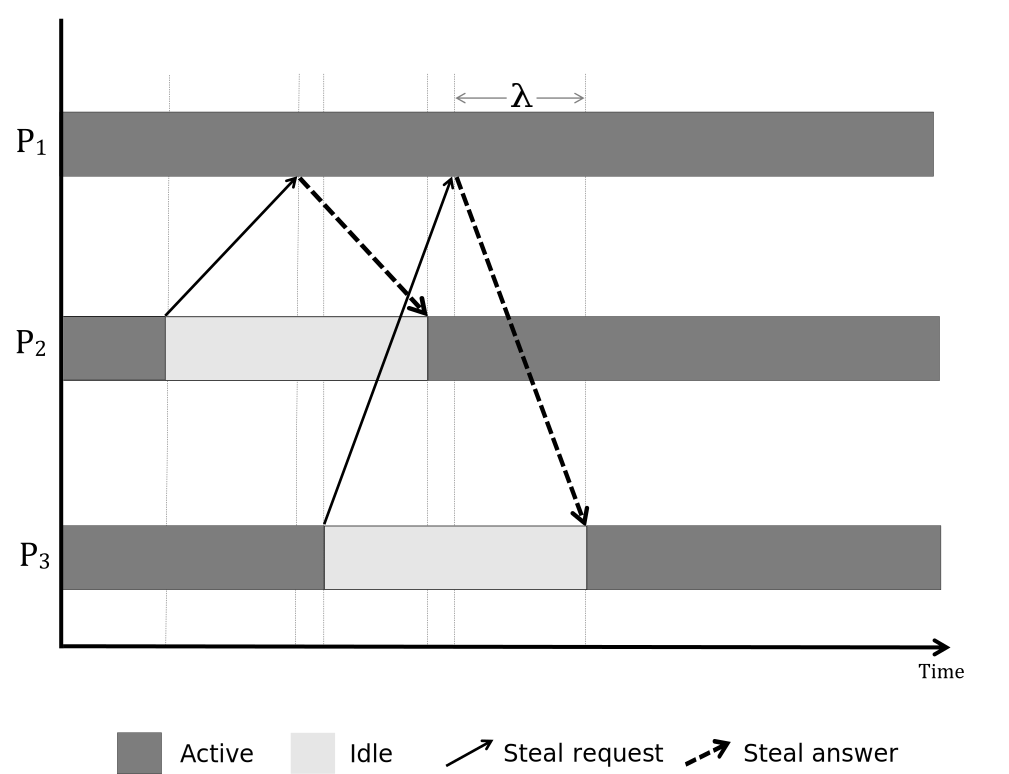
\includegraphics[width=0.6\linewidth]{figures/ws.pdf}
  \caption{Example of a work stealing execution with 3 processors} 
  \label{fig:workStealing}
\end{figure}




We analyze a model of WS algorithm that has the following features:
\begin{itemize}

\item \textbf{Latency:} All communication takes a time
  $\lambda\in\N^+$ that we call the latency.
  Figure~\ref{fig:workStealing} presents an example of Work Stealing
  execution with latency $\lambda$, A work request that is sent at
  time $t-\lambda$ by a thief will be received at time $t$ by the
  victim.  The thief will then receive an answer at time $t+\lambda$.
  As we consider a discrete-time model, we say that a work request
  arrives at time $t$ if it arrives between $t-1$ (not-included) and
  $t$.  This means that at time $t$, this work request is treated. We
  do not assume that the work requests are synchronized.  The number
  of incoming work requests at time $t$ is denoted by
  $R(t)\in\{0,1,\dots,p-1\}$. It is equal to the number of processors
  sending a work request at time $t - \lambda$.  When a processor $i$
  receives a work request from a thief $j$, it sends a part of its
  work to $j$. This communication takes again $\lambda$ units of time.
  The processor $j$ receives the work at time $t+\lambda$.  We denote
  by $s_{i}(t)$ the amount of work in transit from $P_i$ at time $t$.
  At end of the communication $s_{i}$ becomes 0 until another work
  request arrives.
  
\item \textbf{Single work transfer:} We assume that a processor can
  send some work to at most one processor at a time.  While the
  processor sends work to a thief, it replies by a fail response to
  any other work request. Hence, the work request may fail in the
  following cases: (1) when the victim does not have enough work, (2)
  when it is already sending some work to another thief, or (3) when
  the victim receives more than one work request at the same time. In
  the latter, the processor picks random thief and send a negative
  response to the remaining thieves.
  

%\item \textbf{Work division:} DThis division of work depends on the
%  model of dependence:
%  \begin{itemize}
%  \item If all tasks are independent, the victim sends to the thief
%    half of its work: $w_i(t)=(w_i(t)-1)/2$ ad $s_i(t)=w_i(t-1)/2$.
%  \item In the case of the DAG of precedence, a processor can only
%    answer positively if it has two or more activated tasks in its
%    deque. In this case, it sends its tasks that has the largest
%   height.
% \end{itemize}
%
\item \textbf{Steal Threshold:} The main goal of WS is to share work
  between processors in order to balance the load and the speed-up
  execution. In some cases however it might be beneficial to keep
  work locally and answer negatively to some work requests. 
  We assume that if the victim has less than
  %, in the case of independent asks,
  $\lambda$ units of work to execute, the work request fails
  (answering such a work request would increase the makespan as the
  time to answer a request is $\lambda$ units of time).
  %We do not make such an assumption for the case of DAG because
  %we assume that a processor does not know if the computation time
  %of all the tasks that will be activated by its local tasks will
  %be less than $\lambda$.

\item \textbf{Work division:} Since the tasks are independent, we suppose
    that the victim sends to the thief half of its work:
%\begin{equation*}
%    w_i(t)=w_i(t -1)/2 
%\end{equation*}
%and 
%\begin{equation*}
%    s_i(t)=w_i(t-1)/2
%\end{equation*}
  \begin{align*}
        w_i(t)=\frac{w_i(t -1) - 1}2  \qquad\text{ and }\qquad s_i(t)=\frac{w_i(t-1)-1}2.
  \end{align*}
      
\end{itemize} 

\section{Analysis of the Completion Time}
\label{sec:analysis_indep}

This section contains the main result of the paper which is a bound on
the expected makespan. Before presenting the detailed analysis, we
first describe its main steps before jumping into the technical
analysis.
%of the two models (independent tasks and DAG of precedence).

\subsection{General principle}
\label{generalPrinciple}
We denote by $C_{\max}$ the makespan (\emph{i.e.}, total execution
time).  In a WS algorithm, each processor either executes work or tries
to steal work. As the round-trip-time of a communication is $2\lambda$
and the total amount of work is equal to $\calW$ and the number of
processors is $p$, we have
$pC_{\max} \le \calW + 2\lambda\nbworkrequest$ where $p$ is
the number of processors.  This leads to a straightforward bound of
the Makespan:
\begin{equation}
\centering
  \label{Cmax}
  \mathcal{C}_{max}  \leq \frac{\calW}{p} + 2\lambda\frac{\nbworkrequest}{p}
\end{equation}
Note that the above inequality is not an equality because the
execution might end while some processors are still waiting for work.

The key element of our analysis is to obtain a bound on the number of
work requests. For that, we use what we call a potential function that
represents how the tasks are (un)balanced.  We bound the number of
work requests by showing that each event involving a steal operation
contributes to the decrease of the potential.  Our approach is similar
to the one of \cite{Denis2013} but with one additional key difficulty:
communications take $\lambda$ time units. At first, it seems that
longer communications should translate linearly into the time taken by
work requests but this would neglect the fact that longer
communications also reduce the number of work requests.

In order to analyze the impact of $\lambda$, we reconsider the time
division as periods of duration $\lambda$.  We analyze the system at
each time step $k\lambda$ for $k\in\N$.  By abuse of notation, we
denote by $w_i(k)$ and $s_i(k)$ the quantities $w_i(k\lambda)$ and
$s_i(k\lambda)$. % We denote by $\phi_i(k)$ the part of the potential
% linked to processor~$i$ and by $\phi(k) = \sum_i \phi_i(k)$ the
% potential.
We denote the total number of incoming work requests in the
interval $(\lambda(k-1), \lambda k] $ by
$r(k) = \sum_{j=1}^{\lambda}R((k-1)\lambda+j)$ and we denote by
$q(r(k))$ the probability that a processor receives one or more
requests in the interval $(\lambda(k-1), \lambda k]$ (this function
will be computed in the next section). Note that since a steal
requests takes at least $\lambda$ units of time to be answered, we
have $0\le r(k)\le p$.

The key steps of the analysis are as follows:
\begin{enumerate}
\item First, we will define a potential function $\phi(k)$ that is
  such that we can bound the expected decrease of the potential as a
  function of $r(k)$, the number of work requests in the time
  interval $(\lambda(k-1), \lambda k]$:
  \begin{align*}
    \esp{\phi(k+1)\mid r(k)} \le h(r(k))\phi(k). 
  \end{align*}
  This will be done in Lemma~\ref{lem:indep}. 
        %for the case of independent tasks 
        %and \ref{lem:DAG} for the case of DAGs.
\item Second, we will show that this bound implies that the number of
  work requests is upper bounded by $\gamma\log_2\phi(0)$, where
  $\gamma=\max r/(-p\log_2h(r))$. This will be done in
  Lemma~\ref{lem:OfR}. 
\item We will then obtain a bound on the Makespan by using
  Equation~\eqref{Cmax}.
\end{enumerate}
% In the next section, we analyze the decrease of $\phi(k)$ as a
% function of the number of work requests.
% % bound the ratio $\frac{\phi(k+1)}{\phi(k)}$. 
% We show that there exists a function
% $h: \{1 \cdots p\} \rightarrow [0,1]$ depending on the number of
% incoming work requests $r(k)$ in the time interval
% $(\lambda(k-1), \lambda k]$, such that in average, $\phi(k+1)$ is less
% than $h(r(k))\phi(k)$.  Finally, we use this to derive a bound on the
% total number of work requests. By using equation \eqref{Cmax}, we
% obtain a bound on the Makespan.

\subsection{Expected Decrease of the Potential}

Our results are based on the analysis of the decrease of the
potential. The potential at time-step $k\lambda$ is denoted by $\phi(k)$
and is defined as :
\begin{equation}
  \label{eq:potential_indep}
  \phi(k) = 1+\frac{1}{\lambda^2}\sum_{i=1}^{p} \left(w_{i}(k)^{2} + 2s_{i}(k)^{2}\right). 
\end{equation}
We also denote by $\phi_i(k) = w_{i}(k)^{2} + 2s_{i}(k)^{2}$ the
contribution of processor $i$ to the potential (for
$i\in\{1\dots,p\}$).

The rational behind the definition of Equation~\eqref{eq:potential_indep}
is as follows. The potential is maximal when all the work is contained
in one processor which is the potential function at time $0$ and is
equal to $\phi(0) = 1+\mathcal{W}^2/\lambda^2$.  The schedule
completes when the potential reaches $1$.  Up to the multiplicative
factor $1/\lambda^2$, the rest of Equation~\eqref{eq:potential_indep}
is composed in two terms: $\sum_{i=1}^p w_{i}(k)^{2}$ and
$2\sum_{i=1}^ps_{i}(k)^{2}$. These terms serve to measure how
unbalanced is the work.  The first term is only here to ensure that the
potential is never smaller than $1$ (this is a technical condition
that ensures that $\log \phi(k)\ge0$ and that is used in the proof of
Lemma~\ref{lem:OfR}).

The following lemma shows that $\phi(k)$ decreases in expectation with
$k$. In this lemma, we denote by $\mathcal{F}_{k}$ all the events up to the interval
$((k-1)\lambda, k\lambda]$. The notation $ \mathbb{E}[\phi(k+1) \:|\:
\mathcal{F}_{k}]$ indicated the conditional expectation of $\phi(k+1)$
given all information available at time $k$. We show that it can be
upper bounded by a simple function of the potential at time step $k$
and of the number of work requests $r(k)$. 
\begin{lemma}
  \label{lem:indep}
  The expected ratio between $\phi(k+1)$ and $\phi(k)$ knowing
  $\mathcal{F}_{k}$ is bounded by:
  \begin{equation*}
    \mathbb{E}[\phi(k+1) \:|\: \mathcal{F}_{k}] \leq
    h(r(k))\phi(k),
  \end{equation*}
  where the potential is defined as in
  Equation~\eqref{eq:potential_indep} and
  \begin{align}
    \label{eq:h}
    h(r)=\frac34 + \frac14 \left(\frac{p-2}{p-1} \right)^{r}.
  \end{align}
  
  % Where $q(r(k))$ is the probability for a processor to receive one
  % or more requests in the interval $(\lambda(k-1),\lambda k]$ knowing that there are $r(k)$ incoming work requests.
\end{lemma}

\begin{proof}[Sketch of proof]
  Each event related to a steal request decreases the potential:
  \begin{itemize}
  \item When a steal arrives at a processor with $w_i$ jobs,
    approximately $w_i/2$ jobs remain on this processor while $w_i/2$
    jobs go into a term $s_i$. In Equation~\eqref{eq:potential_indep},
    this transforms a $w_i^2$ into $(w_i/2)^2+2(w_i/2)^2=3w_i^2/4$,
    leading to a decrease of potential by a factor $3/4$ for each
    successful steal.
  \item When some work arrive at a processor, a term $s_i$ of
    Equation~\eqref{eq:potential_indep} is transformed into a term
    $w_i$. Because of the factor $2$, in the potential, this
    transforms $2s_i^2$ into $s_i^2$.
  \end{itemize}
  
  The proof of Lemma~\ref{lem:indep} can be obtained by computing the
  probability that a given processor receives a work request. This
  probability depends of the number of work active processors.  The
  full proof is detailed in Appendix~\ref{proof:lem:indep}.
\end{proof}
%The detailed proof is given in \

%\subsubsection{DAG of precedence}
%In the case of DAG, the potential will depend on the maximal height of
%the tasks that a processor has in its lists. Denoting by $h_i(k)$ the
%maximal height of the tasks that processor $i$ has in its deque, we
%define a quantity $w_i(k)$, that we call the potential work of
%processor $i$, as:
%\begin{align*}
%  w_i(k)=\left\{
%  \begin{array}{ll}
%    (2\sqrt{2})^{h_i(k)} & \text{if $P_i$ has two or more tasks in its deque}\\
%    \frac12(2\sqrt{2})^{h_i(k)}& \text{if $P_i$ has only one task in its deque}\\
%    0 & \text{if $P_i$ does not have any tasks}
%  \end{array}
%        \right.
%\end{align*}
%For the tasks in transit, we define the potential work in transit
%$s_i(k)=\frac12(2\sqrt{2})^{h}$, where $h$ is the height of the task
%in transit.
%
%The potential is then defined similarly as in
%Equation~\eqref{eq:potential_indep}:
%\begin{align}
%  \label{eq:potential_DAG}
%  \phi(k) = 1+ \sum_i \phi_i(k)\qquad\text{where }\phi_i(k)=w^2_i(k) + 2s^2_i(k).
%\end{align}

%We are now ready to prove the following lemma, that is an analogue of
%Lemma~\ref{lem:indep} for the case of dependent tasks. 
%\begin{lemma}\label{lem:DAG}
%  For the case of DAG, the expected ratio between
%  $\phi(k+1)$ and $\phi(k)$ knowing $\mathcal{F}_{k}$ is bounded by:
%  \begin{equation*}
%    \mathbb{E}[\phi(k+1) \:|\: \mathcal{F}_{k}] \leq
%    h(r(k))\phi(k),
%  \end{equation*}
%  where the potential is defined as in
%  Equation~\eqref{eq:potential_DAG} and $h(r)$ is as in
%  Lemma~\ref{lem:indep}, \emph{i.e.}, 
%  $h(r)=\frac34 + \frac14 \left(\frac{p-2}{p-1} \right)^{r}$.
%  % Lemma~\ref{lem:indep} also holds when the tasks have a DAG of
%  % precedence, with a potential function $\phi$ defined as in
%  % Equation~\eqref{eq:potential_DAG}. 
%\end{lemma}
%
%\begin{IEEEproof}
%  Similarly to the proof of Lemma~\ref{lem:indep}, we study the
%  expected decrease of the potential by distinguishing three cases:
%  the case $s_i>0$ (work arriving at a thief) and the case where a
%  processor is or becomes idle correspond to cases 1 and 4 of
%  Lemma~\ref{lem:indep} and can be analysis exactly as what was done
%  since Cases~1 and 4 of the proof of Lemma~\ref{lem:indep} do not
%  depend on the task dependence model.  Moreover, the distinction
%  between Case~2 and Case~3 that was done for independent tasks is not
%  necessary for DAGs as there is no steal threshold for DAG. Last, the
%  analysis of Case~2b of Lemma~\ref{lem:indep} is similar: if a
%  processor does not receive any work request, the potential does not
%  grow.
%
%  Hence, in the remainder of the proof, we focus on the only
%  interesting case which what happens when a processor receives one or
%  more work request (Case~2b of the proof of Lemma~\ref{lem:indep}.
%  We distinguish two cases depending on how many tasks are in the
%  deque of processor $i$ when it receives a work request.
%  \begin{enumerate}
%  \item If processor $i$ has only one task (say of height $h$), then
%    it cannot send work. In this case, it will complete
%    its tasks that will activate at most $2$ tasks of height $h-1$. In
%    such a case, the potential work of processor $i$ will go from
%    $w_i(k)=\frac12(2\sqrt{2})^h$ to at most
%    $w_i(k+1)=(2\sqrt{2})^{h-1}$. This shows that 
%    \begin{align*}
%        \phi_i(k+1) &= w^2_i(k+1)\le (2\sqrt{2})^{2h-2} \\
%        &= (2\sqrt{2})^{2h}/8
%      =w_i(k)^2/2 \le \frac12 \phi(k). 
%    \end{align*}
%  \item If processor $i$ has two or more tasks, then by construction,
%    it can have at most two tasks of maximal height (say $h$). In this
%    case, the processor will send one task (of height $h$) to the
%    thief, and will at the mean time execute the other task. In this
%    case, the maximal height of the task of its deque will be $h-1$
%    and the task sent will be of height $h$. This implies that
%    $w_i(k+1)\le (2\sqrt{2})^{2h-1}\le w_i(k)/(2\sqrt2)$ and
%    $s_i(k+1)\le \frac12(2\sqrt{2})^{h}\le w_i(k)/2$. This shows
%    that:
%    \begin{align*}
%        \phi_i(k+1) &= w^2_i(k+1)+2s^2_i(k+1) \\
%        &\le w^2_i(k)/8 +
%        2w^2_i(k)/4\\ 
%        &= \frac58 \phi_i(k). 
%    \end{align*}
%  \end{enumerate}
%  As both $1/2$ and $5/8$ are strictly smaller than the $3/4$ of
%  Equation~\eqref{eq:proof_indep_34}, the rest of the proof of
%  Lemma~\ref{lem:indep} can be applied \emph{mutatis mutandis} to
%  prove Lemma~\ref{lem:DAG}.
%\end{IEEEproof}

\subsection{Analysis of the makespan}
\label{gamma}

We are now ready to prove the bound on the total completion time
$C_{\max}$. To show that, we first obtain a bound on the Number of
Work Requests by using Lemma~\ref{lem:indep}.  Let us define the
constant $\gamma$ as follows:
\begin{equation}
  \label{eq:gamma}
  \gamma \eqde \max_{1 \leq r \leq p } \frac{r}{-p \log_2(h(r))},
\end{equation} 
where $h$ is defined in Equation~\eqref{eq:h}.

\begin{lemma}
  \label{lem:OfR}
  Let $\phi(0)$ denote the potential at time $0$ and let $\tau$ be the
  first time step at which the potential reaches $1$.
  %\begin{align*}
  % $\tau \eqde \min \{k \mathrm{~s.t.~} \forall i \in \{1\dots p\} :
  % \phi(k)=1\}. $
  %\end{align*}
  %Then, for both the independent tasks and the DAG models, the number of incoming work requests until $\tau$,
  Then, the number of incoming work requests until $\tau$,
  $R = \sum_{k=0}^{\tau-1} r(k)$, satisfies:
  \begin{align*}
      (i)\qquad  &\esp{R} \leq p\gamma\log_2\phi(0);  \\
      (ii)\qquad &\Proba{R\ge p\gamma(\log_2\phi(0) + x)} \le {2}^{-x}.
  \end{align*}
  The constant $\gamma$ is such that $\gamma<4.03$.
\end{lemma}

\begin{proof}[Sketch of Proof]
  We detail here an informal proof that assumes that the evolution of
  the potential satisfies $\phi(k+1)\le h(r(k))\phi(k)$ (without the
  conditional expectation of Lemma~\ref{lem:indep}). This allows us to
  make a simpler exposition of the main idea of the proof.  Because of
  the stochastic evolution of $\phi(k)$, the real proof is more
  technical and requires the use of Martingale arguments and of
  Jensen's inequality. It is detailed in Appendix~\ref{proof:lem:OfR}.
  
  Assume that when $r$ steal requests arrive during a time-slot, the
  expected potential is multiplied by $h(r)<1$. If $\tau$ is such that
  $\Phi(\tau)=1$, this shows that if the number of steal requests that
  arrive per time slots $0$ to $\tau-1$ are $r(0)$, $r(1)$,\dots
  $r(\tau-1)$, then $1=\phi(\tau) \le h(r(1))\dots h(r(k)) \phi(0)$,
  which implies that
  $-\log_2 h(r(1))- \dots - \log_2 h(r(k))\le \phi(0)$.  The
  definition of $\gamma$ in Equation~\eqref{eq:gamma} is a worst case
  analysis of what would happen if an adversary could choose the
  $r(k)$. Equation~\eqref{eq:gamma} implies that
  $r(k)\le -\gamma p\log h(r(k))$. This shows that
  $R\le \gamma p \log_2\phi(0)$.
\end{proof}

Lemma~\ref{lem:OfR} provides a bound on the number of work requests
before the end of the schedule. By using Equation~\eqref{Cmax}, this
translates almost immediately into a bound on the makespan, as
summarized by the following theorem.
\begin{theorem}
  \label{theo:cmax}
  Let $C_{max}$ be the Makespan of $\mathcal{W}$ unit independent
  tasks scheduled by WS with latency $\lambda$.  Then,
  \begin{align*}
    (i)  \qquad &\esp{C_{max}} \leq \frac{\mathcal{W}}{p} +  4\lambda\gamma\log_2\frac{\mathcal{W}}{\lambda}  + 2\lambda\gamma;\\
    (ii) \qquad  &\Proba{ C_{max}  \ge \frac{\mathcal{W}}{p} +
                   4\lambda\gamma\log_2\frac{\mathcal{W}}{\lambda}  +
                   x} \le {2}^{-x/(2\lambda\gamma)}. 
  \end{align*}

  %Let $C_{max}$ be the Makespan of $\mathcal{W}$ unit tasks with a DAG
  %of precedence that has a critical path of $D$ scheduled by WS with
  %latency $\lambda$.  Then
  %\begin{align*}
  %  (i)  \qquad &\esp{C_{max}} \leq \frac{\mathcal{W}}{p} +
  %                6\lambda\gamma D  \\
  %  (ii) \qquad  &\Proba{ C_{max}  \ge \frac{\mathcal{W}}{p} +
  %                 6\lambda\gamma D  + x} \le
  %                 {2}^{-x/(2\lambda\gamma)}, 
  %\end{align*}
  The constant $\gamma$ is the same as in Lemma~\ref{lem:OfR}. In
  particular $\gamma<4.03$.
\end{theorem}


\begin{pf}
\label{proof_cmax}
  %Both cases will be proved separately.
  %\emph{Independent tasks} -- 
  By Lemma~\ref{lem:OfR}, the number of
  incoming work requests until $\tau$ is bounded by
  $p\gamma\log_2\phi(0)$, with $\phi(0)=1+\calW^2/\lambda^2$. Moreover
  by definition, the schedule is finished at time $\tau$. Thus by
  Equation~\eqref{Cmax} we have
  \begin{align*}
    \esp{\mathcal{C}_{max}}  \leq \frac{\calW}{p} + 2\lambda
                               \gamma\log_2\left(1+\frac{\calW^2}{\lambda^2}\right)
                              \leq \frac{\calW}{p} + 4\lambda\gamma\log_2\left(\frac{\mathcal{W}}{\lambda}\right) + 2\lambda\gamma,
  \end{align*}
  
  where we used that $\log_2(1+x)\le1+\log_2(x)$ for $x\ge1$.
  
  By the same way, we use Lemma~\ref{lem:OfR}~$(ii)$ and Equation
  \ref{Cmax} we obtain:
  \begin{align*}
      \Proba{ C_{max}  \ge \frac{\mathcal{W}}{p} + 
    4\lambda\gamma\log_2\left(\frac{\mathcal{W}}{\lambda}\right)+4\lambda\gamma+x}
    &\le \Proba{2\lambda \frac{R}{p} \ge
      2\lambda\gamma\log_2\phi(0)+ x}\\
    &=\Proba{R \ge 
      p\gamma \log_2\left(\frac{\mathcal{W}}{\lambda}\right)+p\gamma
      \frac{x}{2\lambda\gamma}}\le {2}^{-x/(2\lambda\gamma)}.
  \end{align*}
  % \emph{DAG of precedence}. The case of DAG is similar, the only
 % difference being the expression of the potential at time $0$. In the
 % case of a DAG, the potential at time $0$ is equal to
 % $1+\frac14(2\sqrt{2})^{2D}=1+\frac148^D\le 8^D$ where $D$ is the
 % critical path.  This shows that $\log_2\phi(0)\le D\log_28=3D$ which
 % implies that
 % \begin{align*}
 %   \esp{\mathcal{C}_{max}}
 %   & \leq \frac{\calW}{p} + 6\lambda\gamma D.  
 % \end{align*}
\end{pf}

%The bounds that we obtained in Theorem~\ref{theo:cmax} are composed of
%a term due to the computation of tasks ($\calW/p$) and an overhead
%term related to the depth.  In case of independent tasks the depth is
%$\log(W)$ but we obtain a slightly better bound due to tasks not being
%divided below $\lambda$.  We actually think bounds on the DAG could be
%refined when considering non-unit tasks.
%
%% to divide the tasks:
%% $\log_2(\calW/\lambda)$ for the independent tasks and the critical
% path $D$ for the case of DAG. For the case of independent tasks, the
% term $\log_2(\calW/\lambda)$ corresponds to the number of divisions
% that are needed to go from a bag of $\calW$ tasks to many chuncks of
% $\lambda$ tasks, which is the size of the chunks that will not be
% divided.  In the case of DAG, the critical path $D$ also corresponds
% to the number of division. As we consider binary DAG, $\log_2\calW$ is
% an analogue of $D$.



%%% Local Variables:
%%% mode: latex
%%% TeX-master: "main"
%%% End:

\section{Experiments Results for Independent tasks}
\label{sec:experiemnts}

In the previous section, we proved a new upper bound of the Makespan
of WS with an explicit latency. The objective of this section is to
study WS experimentally in order to confirm the theoretical results
and to refine the constant $\gamma$. To this end, we developed an
\textit{ad-hoc} simulator that follows strictly the WS model. We focus on
the case of independent tasks. We start by describing this
simulator and the considered test configurations.  Using the
experimental results, we show that the previous theoretical bound is close to
the experimental results.  We conclude with a discussion on where
would the analysis be made more precise. 
%OFinally, we discuss different difficulties of our analyze and the constant factor $4\gamma$ of the $\log_2(\frac{\mathcal{W}}{\lambda})$.


\subsection{Simulator}

Simulation analysis is a very popular and powerful method 
for understanding complex problems when mathematical analysis is unreachable.

For this purpose, there exist many simulators on parallel and distributed computing.
Most of them are developed for specific research projects by researchers and are not well-documented,
and/or no longer maintained. However, there exist several general purpose and high quality simulators
like SimGrid~\cite{SIMGRID} that includes many features: It allows to consider complex
situations like congestion, cache effects for particular architectures, etc.
However, such simulators are usually very computationally expensive,
and it requires a high entry cost to develop in.

Our purpose here is less ambitious since we target simple processing
units. We are interested in observing a simple aspect of the execution process of WS
algorithms on platforms with different topologies.
For these reasons, we developed a lightweight simulator,
%which was designed to be sufficiently flexible in order to simulate different Work Stealing models.
Its flexibility allows us to experiment several variants of WS algorithms,
with different topologies, and different types of application.
The simulator generates also extensive logs for a detailed analysis for each tested scenario.

WS-simulator can run different models of execution under the WS paradigm of an application on a platform. An application
consists of a list of tasks with or without dependencies, and the
platform consists of multiple processors linked by a specific
network/topology.  The simulator allows to execute a scenario with a specific
task on a specific platform. 

The overall architecture of WS-Simulator is composed of six main units (called engines),
that are depicted in Figure~\ref{fig:archsimu}. The event engine is the core of the simulator,
it manages the processors' events during the time to run the simulation of a scenario.
The events are executed through the processor engine, which provides different
functionalities to perform the tested WS algorithm.
The processor engine uses the task engine to manage the execution of the tasks
and it uses the topology engine to manage the interactions between the processors.
During the execution of a simulation, the log engine keeps track of different
information and generates different logs.
More details are available at the website \url{https://wssimulator.github.io}
which describes in detail our simulator and how to use it.

\begin{figure}[h]
  \centering
    \includegraphics[width=0.7\linewidth]{figures/simulatorArchitecture.png} 
  \caption{The overall architecture of WS-simulator}
    \label{fig:archsimu}
\end{figure}


\subsection{Configurations}

For our tests, we configure our WS-simulator in order to follow the model
of independent tasks described in Section~\ref{sec:wsmechanisms} to
schedule $\mathcal{W}$ unitary independent tasks on a distributed
platform composed of $p$ identical processors. The communication
latency between the processors is equal to $\lambda$.  
To ensure reproducibility, this configuration of the simulator is detailed
in WS-Simulator website\footnote{\url{https://wssimulator.github.io/pages/wssimulator-one-cluster.html}}.

\subsection{Validation of the bound and definition of the ``overhead
  ratio''}

% under different parameters $\mathcal{W}$, $p$ and $\lambda$. 


As seen before, the bound of the expected Makespan is the sum of two
terms: The first term is the ratio $\mathcal{W}/{p}$ which does not
depend on the configuration nor on the algorithm; The second term
represents the overhead related to work requests.  Our analysis bounds
the second term to derive our bound on the Makespan.  To analyze the
validity of our bound, we define what we call the \emph{overhead
  ratio} as the ratio between the second term of our theoretical bound
($4\gamma\lambda\log_2(\mathcal{W}/\lambda)$) and the simulated
execution time minus the ratio $\mathcal{W}/p$: for a given
simulation, we define
\begin{align}
  \label{eq:overhead}
  \text{Overhead\_ratio}=\frac{4\gamma\lambda\log_2(\mathcal{W}/\lambda)}
  {\text{Simulated\_execution\_time}  - \frac{\calW}{p}}.
\end{align}

To study this overhead ratio, 
%As said earlier, each simulation is fully described by three
%parameters: $(\calW, p, \lambda)$. For our tests, 
we vary the number of unit tasks $\mathcal{W}$ between $10^5$ and $10^8$, the number of
processors $p$ between 32 and 256 and the latency $\lambda$ between 2
and 500 which is a realistic range of actual systems.
Each experimental setting has been reproduced 1000 times in
order to compute median or interquartile ranges. 


\begin{figure}[ht]
  \centering
  \begin{tabular}{@{}c@{}c@{}c@{}}
    \includegraphics[width=0.33\linewidth]{figures/overheadratioWPinv2.eps}
    
    % \caption{Overhead ratio as a function of $(\mathcal{W},p)$  ($\lambda = 262$)}
    % \label{fig:accuracy}
    % \end{figure}
    % \begin{figure}[tp!]
    %   \centering
    &\includegraphics[width=0.33\linewidth]{figures/overheadratioWPinv262.eps}
    &\includegraphics[width=0.33\linewidth]{figures/overheadratioWPinv482.eps}\\
    (a) Latency $\lambda=2$
    &(c) Latency $\lambda=262$&(d) Latency $\lambda=282$
    
  % \caption{Overhead ratio as a function of $(\mathcal{W},p)$   ($\lambda = 262$)}
%  \label{fig:accuracy}
%\end{figure}
%\begin{figure}[tp!]
%  \centering
  
  
  \end{tabular}
    
  \caption{Overhead ratio (defined in Equation~\eqref{eq:overhead}) as
    a function of $(\mathcal{W},p)$ for different values of
    latency~$\lambda$.}
  \label{fig:accuracy}
\end{figure}


%\begin{figure*}[!t]
%\centerline{\subfigure[Case I]{\includegraphics[width
%=2.5in]{figures/overheadratioWPinv.eps}
%%\label{fig_first_case}}
%%\hfil
%%\subfigure[Case II]{\includegraphics[width=2.5in]{figures/overheadratioWPinv.eps}
%%\label{fig_second_case}}}
% \caption{Simulation results}
%\label{fig_sim}
%\end{figure*}



Figure~\ref{fig:accuracy} plots the overhead ratio according to each
couple $(\mathcal{W}, p)$, for different latency values $\lambda= \{2,\ 262,\ 482\}$
units of time.
%Similar observations have been observed with all values of latency used.
The~x-axis is $(\mathcal{W}, p)$ for all values of $\mathcal{W}$ and $p$ intervals
and the y-axis shows the overhead ratio.
We use here a BoxPlot graphical method to present the
results. BoxPlots provides a good overview and a numerical summary of a
data set.  The ''interquartile range'' in the middle part of the plot
represents the middle quartiles where 50\% of the results are
presented.  The line inside the box presents the median. The whiskers
on either side of the IQR represent the lowest and highest quartiles
of the data.  

We observe that our upper bound is about 4 to 5.5 times greater than
to the one computed by simulation (depending on the range of
parameters). The ratio between the two bounds decreases with the
number of processors but seems fairly independent of $\calW$.


\begin{figure}[htb]
  \includegraphics[width=\linewidth]{figures/analysis.pdf}
  \caption{Evolution of the state of the systems for different
    number of processors ($\lambda=500,\ W=10^7$). Each column
    corresponds to a number of processors ($64$, $128$ or
    $256$).  The first line corresponds to $\phi_{\max}$
    (defined in Equation~\eqref{eq:phi_max}).  The second line
    displays the number of idle processors $r(k)$. The third
    line displays $g(r(k))$ (defined in
    Equation~\eqref{eq:g}). In all figures, the $x$-axis
    corresponds to the number of time steps $k$.}
  \label{fig:exp_analysis}
\end{figure}

\subsection{Discussion : where does the overhead ratio come from?}

The challenge of this paper is to analyze WS algorithm with an
explicit latency.  We presented a new analysis which derives a bound
on the expected Makespan for a given $\mathcal{W}$, $p$ and~$\lambda$.
It shows that the expected Makespan is bounded by $\calW/p$ plus an
additional term bounded by $4\gamma\lambda\log_2(\calW/\lambda)$ with
$4\gamma\approx16$.  As observed in Figure~\ref{fig:accuracy}, the
constant $4\gamma$ is about four to five times larger than the one
observed by simulation. A more precise fitting based on simulation
results leads to the expression
$\mathcal{W}/p + 4\lambda\log_2(\mathcal{W}/\lambda)$ (the value $4$
is an average over all our experiments). We explain below where does
the discrepancy between the theoretical bound of $16$ and the
experimental result of $4$ come from by looking at the different steps
of the proof.  Our analysis makes essentially three approximations:
-1) The function $h(r)$ is an upper bound on the potential diminution.
-2) We consider a worst case scenario for the number of steal requests
when we define $\gamma=\max_rg(r)=g(p-1)$; and (3) We bound $\gamma$
by $4.03$.  We review below the contribution of each approximation to
the overhead ratio.

To illustrate our explanations, we run three simulations by using our
simulator and report the results in Figure~\ref{fig:exp_analysis}.
These three executions have the same number of tasks $W=10^7$ and
latency $\lambda=500$ and we consider three values of processors:
$p\in\{64,\ 128,\ 256\}$. This figure illustrates the evolution with
time of the potential $\phi(k)$, the number of idle processors and the
value of $\gamma$ defined in section~\ref{gamma}. Each column
represents a value of $p$.  The lines represent the results for each
metric.


% Now, we briefly review the different approximation in order to explain
% the role of each approximation in the overhead ratio.

\subsubsection{Impact of the bound $h(r)$}
The first step of our analysis is to prove a bound on the decrease
potential: We show in Lemma~\ref{lem:indep} that
\begin{align}
  \label{eq:phi_exp}
  \esp{\Phi(k+1) \mid \calF_t} \le h(r(k)) \Phi(k). 
\end{align}

This bound is obtained by computing the diminution of the potential in
the various cases of the proof of Lemma~\ref{lem:indep}.  These various
cases make different approximations. First, our bound $h(r)$ is the
maximum between the ratio $2/3$ of Case~1 and the 
ratio $h(r)$ of Case~2a. Second, we assumed that we do not know when a
work requests arrive in the interval.  We therefore always took the
worst case (arrivals at the end of the intervals). Third, we neglect
the diminution of the potential due to working processors (Case~2a).

To see measure the impact of this approximation, we define a
theoretical function $\phi_{\max}(k)$ that would corresponds to the
potential of the system if the inequality of
Equation~\eqref{eq:phi_exp} was an equality:
\begin{equation}
  \label{eq:phi_max}
  \phi_{\max}(k) =
  \begin{cases*}
    \phi(0) & if $k = 0$, \\
    h(r(k))\phi_{\max}(k-1)        & otherwise.
  \end{cases*}
\end{equation}

In Figure~\ref{fig:exp_analysis}-(Line~1), we plot this theoretical
function and the real potential function as a function of time step
$k$. This figure indicates that the distance between the real
potential and the theoretical bound is relatively small at the
beginning of the execution, which makes sense since the diminution of
the potential is dominated by the diminution related to Case~2a. The
two function starts diverging slowly in the middle of the execution
and this divergence is accentuated at the end: when the execution is
close to finishing, the actual potential decreases much faster that
its bound. We believe that this divergence is mostly due to neglecting
the diminution of potential due to working processors: At the
beginning of the execution when all processors have many tasks to
execute, neglecting working processors is negligible; At the end of the
execution when the remaining work is small, the potential diminution
is greatly affected by the working processors.  Our analysis could be
tightened by taking a more complex potential function that will take
more carefully the impact of working processors.
% We do not believe, however, that there is an easy way to do so.

\subsubsection{Evolution of the number of work requests}

In our analysis, we study how the potential decreases a function of
the number of steal requests $r(k)$. To obtain a bound, we then use a
worst-case analysis and define $\gamma$ as the maximal of a function
$g(r)=r/(-p\log_2h(r))$: $\gamma=\max_r g(r)$. As shown in
Figure~\ref{fig:g}, $g(r)$ is between $2.8$ where $r$ is small to $4$
when $r$ is large.  On the second Line~2 of
Figure~\ref{fig:exp_analysis}, we depict how the number of idle
processors evolve over time. We observe that an execution has
essentially three phases: At the beginning, there is a high number of
idle processors since the work has to be divided among processors; In
the middle of the execution, the number of idle processors is small as
everybody is working.  In the final execution phase, it increases as
finding work becomes harder.


In Figure~\ref{fig:exp_analysis}-(Line~3), we plot $g(r(k))$ and
$\gamma$ as a function of the time step $k$.  The figure shows that
$g(r(k))$ is often about $2.8$ (because the period where the number of
idle processors is low is long). This suggests that our bound
$\gamma=\max_r g(r)$ is about $1.4$ times too high. Being able to
capture more precisely how the number of idle processors evolves might
lead to a bound that would be around $30\%$ times smaller.

\subsubsection{Bound $\gamma<4.03$ and impact of the number of
  processors}

In our analysis, we show that $\gamma=g(p-1)$ and we bound $\gamma$ by
$4.03$. In fact, the value of $4.03$ corresponds to what happens when
$p$ goes to infinity but smaller values of $p$ leads to smaller values
of $\gamma$. This explains why in Figure~\ref{fig:accuracy}, we
observe that the overhead ratio decreases with the number of processors,
from around $5$ for $32$ processors to around $4$ to $4.5$ for $256$
processors.


\medskip

In our simulation, we observe that the overhead ratio is between $4$
to $5$. Based on our experimental study of the evolution of the number
of work requests with time, we believe that the worst-case analysis
$\gamma=g(p-1)$ and the bound of $4.03$ contributes to a factor of
about $1.5$ of the overhead ratio. The remaining factor (of about $3$)
is mostly due to the bound $h$ that we obtained in
Lemma~\ref{lem:indep}. Refining this lemma, for example by being able
to estimate the decrease of potential due to the work execution or by
using a different potential definition, would lead to a tighter bound.




%%% Local Variables:
%%% mode: latex
%%% TeX-master: "main"
%%% End:

% !TEX root = ./main.tex
\section{Extension to a Model of Tasks with Precedence}
\label{sec:dagOfPrecedence}
%\subsubsection{DAG of precedence}

In this section, we show that the analysis presented in
Section~\ref{sec:analysis_indep} can be adapted to the case of tasks
with precedence constraints. The main difficulty here is to
redefine a new potential function, which we do by combining the ideas
of \cite{Arora2001,Denis2013} to our model of latency of
Section~\ref{sec:analysis_indep}. This demonstrates the power of an
approach by potential function. 

\subsection{Model}

We consider a model similar to \cite{Arora2001,Denis2013} where the
workload is composed of $\mathcal{W}$ unitary tasks that have
precedence constraints represented by a DAG (Directed Acyclic Graph). 
This DAG has a single source that represents the first task and that
is originally located on a given processor.
We consider that the scheduling is done as in
\cite{Arora2001}: each processor maintains a double-ended queue
(called deque) of activated tasks. If a processor has one or more task
in its deque, it executes the task at the head of its deque. This
takes one unit of time. After completion, a task might activates $0$,
$1$ or $2$ tasks that are pushed at the end of the deque.  The
activation tree is a binary tree whose shape depends on the execution
of the algorithm. It is a subset of the original DAG and has the same
critical path.  We define the height of node of this tree as
follows. The height of the source as $D$ (\emph{i.e.}, the length of
the critical path). The height of another task is equal to the length
of its father minus one.  We assume that when a processor steals work
from another processor, it steals the activated tasks with the largest
height.  In the case of the DAG of precedence, a processor can only
answer positively if it has two or more activated tasks in its deque.
In this case, it sends its task that has the largest height.

\subsection{Potential function}
The potential will depend on the maximal height of
the tasks that a processor has in its lists. Denoting by $h_i(k)$ the
maximal height of the tasks that processor $i$ has in its deque, we
define a quantity $w_i(k)$, that we call the potential work of
processor $i$, as:
\begin{align*}
  w_i(k)=\left\{
  \begin{array}{ll}
    (2\sqrt{2})^{h_i(k)} & \text{if the processor
                           $i$ has two or more tasks in its deque,}\\
    \frac12(2\sqrt{2})^{h_i(k)}& \text{if the processor
                                 $i$ has only one task in its deque,}\\
    0 & \text{if the processor
        $i$ does not have any tasks.}
  \end{array}
        \right.
\end{align*}
For the tasks in transit, we define the potential work in transit
$s_i(k)=\frac12(2\sqrt{2})^{h}$, where $h$ is the height of the task
in transit.

The potential is then defined similarly as in
Equation~\eqref{eq:potential_indep}:
\begin{align}
  \label{eq:potential_DAG}
  \phi(k) = 1+ \sum_i \phi_i(k)\qquad\text{where }\phi_i(k)=w^2_i(k) + 2s^2_i(k).
\end{align}
We are now ready to prove the following lemma, that is an analogue of
Lemma~\ref{lem:indep} for the case of dependent tasks. 
\begin{lemma}\label{lem:DAG}
  For the case of DAG, the expected ratio between
  $\phi(k+1)$ and $\phi(k)$ knowing $\mathcal{F}_{k}$ is bounded by:
  \begin{equation*}
    \mathbb{E}[\phi(k+1) \:|\: \mathcal{F}_{k}] \leq
    h(r(k))\phi(k),
  \end{equation*}
  where the potential is defined as in
  Equation~\eqref{eq:potential_DAG} and $h(r)$ is as in
  Lemma~\ref{lem:indep}, \emph{i.e.}, 
  $h(r)=\frac34 + \frac14 \left(\frac{p-2}{p-1} \right)^{r}$.
% Lemma~\ref{lem:indep} also holds when the tasks have a DAG of
% precedence, with a potential function $\phi$ defined as in
% Equation~\eqref{eq:potential_DAG}. 
\end{lemma}
\begin{pf}
  Similarly to the proof of Lemma~\ref{lem:indep}, we study the
  expected decrease of the potential by distinguishing three cases:
  the case $s_i>0$ (work arriving at a thief) and the cases where a
  processor is or becomes idle correspond to cases 1 and 4 of
  Lemma~\ref{lem:indep} and can be analyzed exactly as what was done
  since Cases~1 and 4 of the proof of Lemma~\ref{lem:indep} do not
  depend on the task dependence model.  Moreover, the distinction
  between Case~2 and Case~3 that was done for independent tasks is not
  necessary for DAGs as there is no steal threshold for DAG. Last, the
  analysis of Case~2b of Lemma~\ref{lem:indep} is similar: if a
  processor does not receive any work request, the potential does not
  grow.

  Hence, in the reminder of the proof, we focus on the only
  interesting case which what happens when a processor receives one or
  more work request (Case~2b of the proof of Lemma~\ref{lem:indep}).
  We distinguish two cases depending on how many tasks are in the
  deque of processor $i$ when it receives a work request.
  \begin{enumerate}
  \item If processor $i$ has only one task (say of height $h$), then
    it cannot send work. In this case, it will complete
    its tasks that will activate at most $2$ tasks of height $h-1$. In
    such a case, the potential work of processor $i$ will go from
    $w_i(k)=\frac12(2\sqrt{2})^h$ to at most
    $w_i(k+1)=(2\sqrt{2})^{h-1}$. This shows that 
    \begin{align*}
      \phi_i(k+1) = w^2_i(k+1)\le (2\sqrt{2})^{2h-2} = (2\sqrt{2})^{2h}/8 
      = w_i(k)^2/2 \le \frac12 \phi_i(k). 
    \end{align*}
  \item If processor $i$ has two or more tasks, then by construction,
    it can have at most two tasks of maximal height (say $h$). In this
    case, the processor will send one task (of height $h$) to the
    thief, and will at the mean time execute the other task. In this
    case, the maximal height of the task of its deque will be $h-1$
    and the task sent will be of height $h$. This implies that
    $w_i(k+1)\le (2\sqrt{2})^{2h-1}\le w_i(k)/(2\sqrt2)$ and
    $s_i(k+1)\le \frac12(2\sqrt{2})^{h}\le w_i(k)/2$. This shows
    that:
    \begin{align*}
      \phi_i(k+1) = w^2_i(k+1)+2s^2_i(k+1) \le w^2_i(k)/8 + 2w^2_i(k)/4 
      = \frac58 \phi_i(k). 
    \end{align*}
  \end{enumerate}
  As both $1/2$ and $5/8$ are strictly smaller than the $3/4$ of
  Equation~\eqref{eq:proof_indep_34}, the rest of the proof of
  Lemma~\ref{lem:indep} can be applied \emph{mutatis mutandis} to
  prove Lemma~\ref{lem:DAG}.
\end{pf}

\subsection{Analysis of the Makespan}
\label{subsec:analysisMakspan}


% \subsection{Bound on the Number of Work Requests}
% \label{def:gamma}

The bound on the expected decrease of the potential of
Lemma~\ref{lem:DAG} is the same  as the bound of Lemma~\ref{lem:indep}
for independent tasks. Since the proof of Lemma~\ref{lem:OfR} does not depend on the dependence
structure of the tasks but only the bound on the expected decrease of
Lemma~\ref{lem:indep}, this implies that Lemma~\ref{lem:OfR} also
applies for the case of tasks with precedence.

We are now ready to prove the bound on the total completion time
$C_{\max}$ for the DAG model that is summarized by the following theorem:
\begin{theorem}
  \label{theo:dag_cmax}
  Let $C_{max}$ be the Makespan of $\mathcal{W}$ unit tasks with a DAG
  of precedence that has a critical path of $D$ scheduled by WS with
  latency $\lambda$.  Then
  \begin{align*}
    (i)  \qquad &\esp{C_{max}} \leq \frac{\mathcal{W}}{p} +
                  6\lambda\gamma D; \\
    (ii) \qquad  &\Proba{ C_{max}  \ge \frac{\mathcal{W}}{p} +
                   6\lambda\gamma D  + x} \le
                   {2}^{-x/(2\lambda\gamma)}.
  \end{align*}
  The constant $\gamma$ is the same as in Lemma~\ref{lem:OfR}. In
  particular $\gamma<4.03$.
\end{theorem}
\begin{pf}
  The case of DAG is similar as the independent tasks model %(proof~\ref{proof_cmax}),
  the only difference being the expression of the potential at time $0$.
  In the case of a DAG, the potential at time $0$ is equal to
  $1+\frac14(2\sqrt{2})^{2D}=1+\frac148^D\le 8^D$ where $D$ is the
  critical path.  This shows that $\log_2\phi(0)\le D\log_28=3D$ which
  implies that
  \begin{align*}
    \esp{\mathcal{C}_{max}}
    & \leq \frac{\calW}{p} + 6\lambda\gamma D.
  \end{align*}
\end{pf}
The bounds that we obtained in Theorem~\ref{theo:dag_cmax} and Theorem~\ref{theo:cmax} are composed of
a term due to the computation of tasks ($\calW/p$) and an overhead
term related to the depth.  In case of independent tasks the depth is
$\log(W)$ but we obtain a slightly better bound due to tasks not being
divided below $\lambda$.  We actually believe that the bounds on the DAG could be
refined when considering non-unit tasks.


%%% Local Variables:
%%% mode: latex
%%% TeX-master: "main"
%%% End:


\section{Conclusion}
\label{sec:conclusion}

We presented in this paper a new analysis of Work Stealing algorithm
where each communication has a latency of $\lambda$.  Our main result
was to show that the expected Makespan of a load of $\calW$ independent
tasks on a cluster of $p$ processors is bounded by
$\calW/p+16.12\lambda\log_2(\calW/\lambda)$. Our analysis makes use of
potential functions whose expected decrease per unit time can be
bounded as a function of the number of work requests. We then use this
to derive a theoretical upper bound on the expected makespan. We also
extend this analysis one step further, by providing a bound on the
probability to exceed the bound of the makespan.  We showed also that
we can extend the same analysis for a model of tasks with precedence.

To assess the tightness of this analysis we developed an
\textit{ad-hoc} simulator. We showed by comparing the theoretical
bound and the experimental results that our bound is realistic.  We
observed moreover that our bound (established on worst case analysis)
is four to five times greater than the experimental results and it is
stable for all the tested values. By using traces of execution, we
quantify the various approximations that are made in the analysis and
suggest where the analysis could be made more accurate.

For future work, we intend to study work stealing strategies in
complex topologies where the latency can depend on the topology.  This
work is a first step towards this as it allows a full understanding of
the work stealing in the basic, homogeneous, setting.






%\bibliographystyle{IEEEtran}



\bibliographystyle{cas-model2-names}
%\bibliographystyle{model1-num-names}
%\bibliography{biblio}
% Loading bibliography database
\bibliography{cas-refs}

\appendix
\section{Technical Proofs}
\label{sec:proofs}

\subsection{Proof of Lemma~\ref{lem:indep}}
\label{proof:lem:indep}

%\begin{pot}
  To analyze the decrease of the potential function, we distinguish
  different cases that corresponds to processors that are executing
  work, sending or answering work requests.  We show that each case
  contributes to a diminution of the potential.

  Between time $k\lambda$ and $(k+1)\lambda$, a processor does (at
  least) one the following four things.  These cases cover all
  possible behaviors of the processor.
  % \begin{enumerate}
  % \item The processor is executing and sending work.
  % \item The processor is executing work and available to respond to the work requests sent by idle processors.
  % \item The processor is executing work and will be idle soon.
  % \item The processor is idle.
  % \end{enumerate}
  % We analyse below how much each case contributes to the decrease of
  % the potential.
  \begin{cases}
  \item ($s_i>0$) The processor started to send work to another (idle)
    processor $j$ before time $k\lambda$.  This means that 
    processor $j$ will receive $s_i(k)$ tasks at a time
    $t<(k+1)\lambda$. Note that by assumption, $s_i(k)\ge w_i(k)$
    because processor $i$ has executed some if its own work since
    it started to send half of its work to $j$.  There are two 
    subcases:
    \begin{itemize}
    \item \textbf{Case~1a}. If no additional work requests have been
      received between $t$ and $(k+1)\lambda$, it holds that
      \begin{align*}
        &w_i(k+1)\le w_i(k)\\
        &w_j(k+1)\le s_i(k)\\
        &s_i(k+1)=s_j(k+1)=0. 
      \end{align*}
      This implies that the potential of $i$ and $j$ at time step
      $k+1$ satisfies:
      \begin{align*}
        \phi_i(k+1)+\phi_j(k+1)
        &= w_i(k+1)^2 + w_j(k+1)^2 + 2(s_i(k+1)^2+s_j(k+1)^2) \\
        &\le w_i(k)^2 + s_i(k)^2 \\
        &= w_i(k)^2 + 2s_i(k)^2-s_i(k)^2\\
        &\le \frac23\phi_i(k)\\
        &= \frac23(\phi_i(k)+\phi_j(k)).
      \end{align*}
      The last inequality holds because
      $w_i(k)^2 + 2s_i^2(k)=\phi_i(k)$ and
      $s_i^2(k)=(s_i^2(k)+2s^2_i(k))/3\ge(w^2_i(k)+2s^2_i(k))/3=\phi_i(k+1)/3$. The
      last equality holds because $\phi_j(k)=0$. 
      
    \item \textbf{Case~1b}. If one or more work request has been
      received between $t$ and $(k+1)\lambda$ (by either processor $i$
      or $j$), then this processor will send some of its work of this
      processor. It should be clear that this will further decrease
      the potential (see Case~2b below).
      This shows the inequality :
      \begin{align*}
        \phi_i(k+1)+\phi_j(k+1) \le \frac23(\phi_i(k)+\phi_j(k))
      \end{align*}
      also holds in this case.
    \end{itemize}
    Note that if $w_i<\lambda$, processor $i$ might become idle before
    $(k+1)\lambda$. In this case, it will send a work request. This
    will not modify the potential as the work request will be received
    after time $(k+1)\lambda$.
  \item ($s_i=0$ and $w_i\ge2\lambda$) The processor has work and it is
    available to respond to work requests. We distinguish two cases:
    (case 2a) if this processor receives one or more requests or (case
    2b) if it does not receive any request.
    
    \begin{itemize}
    \item \textbf{Case 2a} -- If processor $i$ receives one or
      more work requests between $k\lambda$ and $(k+1)\lambda$, it
      will respond positively to one processor (say processor $j$)
      by sending it half of its work. All other work requests will
      fail. This implies that $w_i(k+1) \leq w_i(k)/2$ and
      $s_i(k+1)\le w_i(k)/2$ and $w_j(k+1)=s_j(k+1)=0$, which implies
      that
      \begin{equation}
        \label{eq:proof_indep_34}
            \begin{aligned}
              \phi_i(k+1) &= w_i^2(k+1)+2s_i^2(k+1)\\
              &\leq \frac34w_i^2(k)\\
              &=\frac34\phi_i(k).
             \end{aligned}
      \end{equation}
    \item \textbf{Case 2b} -- If processor $i$ does not receive any
      work requests, it will only execute work, in which case
      $\phi_i(k+1)\le\phi_i(k)$
    \end{itemize}
    A given idle processor will choose processor~$i$ as its victim
    with probability $1/(p-1)$. Hence, if $r(k)$ processors sent a
    work requests between $(k-1)\lambda$ and $k\lambda$, then
    processor~$i$ will receive no work requests between $k\lambda$ and
    $(k+1)\lambda$ with probability $((p-2)/(p-1))^{r(k)}$. This shows that
    Case~2a occurs with probability $1-((p-2)/(p-1))^{r(k)}$ while Case~2b
    occurs with probability $((p-2)/(p-1))^{r(k)}$. Hence
    \begin{align*}
      \esp{\phi_i(k+1) \mid \calF_k} &\le \phi_i(k)\left[ \left(\frac{p-2}{p-1}\right)^{r(k)}
                                       +  \frac34\left(1-\left(\frac{p-2}{p-1}\right)^{r(k)}\right)\right]\\
        &=h({r(k)})\phi_i(k). 
    \end{align*}

  \item ($s_i=0$ and $\lambda\le w_i<2\lambda$) The processor has less
    than $2\lambda$ units of work and therefore may or may not be able
    to answer work requests depending if they arrive before its
    remaining work is 
    less than $\lambda$ units of work. If a work request is received
    then we fall back to Case~2a. Otherwise, the processor only
    executes work and
    \begin{align*}
        \phi_i(k+1) &= (\max(0,w_i(k)-\lambda))^2 \\
                    & \le \frac12w_i(k)^2\\
                    &=\frac12\phi_i(k). 
    \end{align*}
   
    % .  To compute $q(r(k))$, we observe
    % that $P_i$ receives zero work requests if the $r(k)$ thieves choose
    % another processor.  Each of these events is independent and
    % happens with probability $\frac{p-2}{p-1}$.  Hence, the
    % probability that $P_i$ receives one or more work requests is~:
    % \label{Procavailable}
    % \begin{equation}
    %   q(r(k)) = 1 - \left(\frac{p-2}{p-1} \right)^{r(k)}
    %   \label{proba}
    % \end{equation}
    % This shows that the ratio of potential in this scenario is:
    % \begin{equation*}
    %   \frac{ \phi_i(k+1)} { \phi_i(k)} \leq \frac{3}{4}q(r(k)) + (1-q(r(k))) \leq 1 - \frac{q(r(k))}{4}
    % \end{equation*} 
    %Where $i\in case2$ means that $P_i$ contributes in $case$ $2$
    
%   \item \textbf{:} $P_i$ with little amount of work
%     $w_i(k) \leq \lambda$ and $s_i(k) = 0$, in this case $P_i$ will
%     respond negatively to any work requests and the potential function
%     goes to $0$ and generates a ratio equal to $0$
% \label{littleWork}

  \item ($s_i=0$ and $w_i<\lambda$) If  processor $i$ is idle or
    became idle between $k\lambda$ and $(k+1)\lambda$, there are two
    sub-cases. The first one is if this processor receives some work
    between $k\lambda$ and $(k+1)\lambda$. In this case this processor
    is the processor $j$ of the Case~1 above and its contribution to
    the potential has already been taken into account. The second one
    is if this processor does not receive work during $k\lambda$ and
    $(k+1)\lambda$ in which case its potential is $\phi_i(k+1)=0$.
  \end{cases}

  Note that in addition to all this decrease, at least one processor
  executed $\lambda$ units of work during $[k\lambda,(k+1)\lambda)$
  (otherwise there would be nothing to compute and the schedule would
  be finished).  This contributes to the decrease of (at least)
  $\lambda^2/3$ to one of the $\phi_i(k)$.

Using the variation of each of these scenarios we find that the expected
potential time $k+1$ is bounded by:
\begin{align*}
    \mathbb{E}[\phi(k+1)\:|\: \mathcal{F}_{k}] &\leq 1+\frac1{\lambda^2}\Bigg( - \frac{\lambda^2}{3}
    + \sum_{i \in \text{Case~1}}\frac{2}{3}\phi_i(k)
      + \sum_{i \in\text{Case~2}}h(r(k))\phi_i(k)  + \sum_{i \in
      \text{Case~3}}\frac{1}{2}\phi_i(k)
      + \sum_{i \in \text{Case~4}} 0 \Bigg) \\
    &\leq \max\left(\frac{2}{3},h(r(k)),\frac{1}{2},0\right)\phi(k)\\
    &= h(r(k))\phi(k),
\end{align*}
  where the last equality holds because $h(r(k))\ge3/4\ge2/3$. 
%   , we have :
% \begin{equation*}
% \max\left(\frac{2}{3},(1-\frac{q(r(k))}{4})\right) = 1-\frac{q(r(k))}{4}
% \end{equation*}
% Then,
% \begin{equation*}
% \mathbb{E}[\phi(k+1)\:|\: \mathcal{F}_{k}] \leq (1-\frac{q(r(k))}{4})\phi(k)  \qedhere
% \end{equation*}
%\end{pot}

\subsection{Proof of Lemma~\ref{lem:OfR}}
\label{proof:lem:OfR}

\subsubsection{Expected number of work requests}

  By definition of $\gamma$, for a number of work requests
  $r\in\{0,\dots,p-1\}$, we have
  $\log_2(h(r)) \leq \frac{r}{ -p \gamma }$ which implies that
  $h(r)\le 2^{-r/(p\gamma)}$.
  % \begin{align*}
  %   \esp{\phi(k+1) \mid \calF_k}&\le h(r(k))\phi(k)\\
  %   &\le \phi(k)2^{-r(k)/(p\gamma)}. 
  % \end{align*}
  Let $X_{k}=\phi(k)\prod_{i=0}^{k-1}2^{r(i)/(p\gamma)}$. By
  Lemma~\ref{lem:indep}, this shows that
  \begin{align*}
    \esp{X_{k+1}\mid\calF_k} &= \esp{\phi(k+1) \mid \calF_k}
                               \prod_{i=0}^{k}2^{r(i)/(p\gamma)}\\
                             &\le \phi(k) 2^{-r(k)/(p\gamma)}
                               \prod_{i=0}^{k}2^{r(i)/(p\gamma)}\\
                             &=X_k.
  \end{align*}
  This shows that $(X_k)_k$ is a supermartingale for the filtration
  $\calF$. As $\tau$ is a stopping time for the filtration $\calF$,
  Doob's optional stopping theorem (see \emph{e.g.},
  \cite[Theorem~4.1]{durrett1996probability}) implies that
  \begin{equation}
    \esp{X_\tau} \le \esp{X_0}. 
    \label{eq:doob}
  \end{equation}
  By definition of $X$, we have $X_0=\phi(0)$ and
  $X_\tau=\phi(\tau)2^{R/(p\gamma)}$. As $\phi(\tau)=1$, this implies
  that
  \begin{align}
    \esp{2^{R/(p\gamma)}}=
    \esp{\phi(\tau)2^{R/(p\gamma)}} \le \phi(0).
    \label{eq:doob2}
  \end{align}
  % As $\phi(\tau)=1$, the above equation implies that
  % $\esp{2^{R/(p\gamma)}}\le\phi(0)$. 
  % Recall that $\tau$ is the first interval in which each processor has
  % an amount of work less than~$3\lambda$, $\tau = \min$\{$k$:
  % $\forall i \in [1,p] $ : $ w_i(k) \leq 3\lambda $\}.  This means
  % that at $\tau-1$, there exists at least one processor $i$ with
  % $w_i(\tau-1) > 3\lambda$.  If this processor received a work
  % request between $\tau-1$ and $\tau$, we have
  % $w_i(\tau) \geq \lambda$. If this processor did not receive a work
  % request between $\tau-1$ and $\tau$, we have
  % $w_i(\tau)>2\lambda$. This implies that
  %  \begin{equation*}  
  %    \phi(\tau) \ge\phi_i(\tau) \ge w_i^2(\tau) + 2s_i^2(\tau) \geq
  %    4\lambda^2 \qquad\mathrm{a.s.}
  %  \end{equation*}
  %  Plugging this into Equation~\eqref{eq:doob2} shows that 
  %  \begin{align}
  %    \esp{2^{R/(p\gamma)}} \le \frac{\phi(0)}{4\lambda^2}.
  %    \label{eq:doob3}
       %      \end{align}
  By Jensen's inequality (see \emph{e.g.},
  \cite[Equation~(3.2)]{durrett1996probability}), we have
  $\esp{R/(p\gamma)}\le\log_2\left(\esp{2^{R/(p\gamma)}}\right)$. This
  shows that
  \begin{align*}
       \esp{R} &\le p\gamma \log_2\phi(0).
   \end{align*}
   Moreover, by Markov's inequality, Equation~\eqref{eq:doob2} implies
   that for all $a>0$:
   \begin{align*}
     \Proba{2^{R/(p\gamma)}\ge a} \le \frac{\phi(0)}{a}.
   \end{align*}
   
   % This implies that
   By using $a=\phi(0)2^{x}$, this implies that $\Proba{R \ge p\gamma (\log_2 \phi(0)  + x) } \le 2^{-x}$.
   % \begin{align*}
   %     \Proba{R \ge p\gamma (\log_2 \phi(0)  + x) } \le 2^{-x}
   %   % &=
   %   %   \Proba{2^{R/p\gamma} \ge (W/2\lambda)^2 2^{x/(p\gamma)}} \le  2^{-x/(p\gamma)}
           %      \end{align*}

 \begin{figure}[t]
   \centering
   \includegraphics[width=.7\linewidth]{figures/g64}
   \caption{Function $g(r)$ as a function of the number of idle
     processor $r$ for $p=\{64,128\}$ processors. We observe that $g$ is
     increasing and upper bounded by $4.03$. }
   \label{fig:g}
 \end{figure}

 \bigskip

 \subsubsection{Bound $\gamma<4.03$}
 % \begin{lemma}
 % \label{gammabound}
 % \end{lemma}
 % \begin{pf}
   Let define the function $g$ as
   \begin{align}
     \label{eq:g}
     g(r)=\frac{r}{-p\log_2\left(\frac34+\frac14\Big(\frac{p-2}{p-1}\Big)^{r}\right)}.
   \end{align}
   
   By definition, the constant $\gamma$ is the maximum of $g$:
   \begin{align*}
     \gamma=\max_{1\le r \le p-1}g(r).  
   \end{align*}
   
   The function $g$ is displayed in Figure~\ref{fig:g} for the case of
   $64$ processors and $128$ processors. As we observe on this curve,
   $g$ is increasing and is thus bounded by $g(p-1)<4.03$.  This is what we
   prove in the remainder of this proof.

   Let $x=(p-2)/(p-1)$ and $y=x^r$, we have $y\in(0,1)$. We have
   \begin{align*}
     \frac{1}{g(r)} = -p\frac{\log_2(3/4+y/4)}{\log_x(y)} =
     -\frac{p\log x}{\log 2} f(y),
   \end{align*}
   where $f(y)=\log(3/4+y/4)/\log(y)$. The first derivative of $f$ is
   \begin{align*}
     f'(y)=\frac{y\log y - (3+y)\log(3/4+y/4)}{y(3+y)(\log y)^2}.
   \end{align*}
   
   The first derivative of the numerator of $f'(y)$ is
   $\log y - \log (3/4+y/4)$ which is negative for $y<1$. Thus it implies
   that $f'(y)$ is decreasing. As $f'(1)=1$, this shows that
   $f'(y)\ge0$ and therefore that $f$ is increasing. This implies that
   $g(r)$ is increasing (because $y$ is decreasing in $r$ and
   $g(r)=\alpha /f(y)$ for $\alpha=-\log 2 / (p\log x) > 0$).

   As $g$ is increasing, $\gamma = g(p-1)$. Now, for all $ p \geq 2$:
   \begin{align*}
       \left(\frac{p-2}{p-1}\right)^{p-1} & = \left( 1 - \frac{1}{p-1}
     \right)^{p-1}\\
       &= \exp \left((p-1)\ln(1-\frac{1}{p-1}) \right)\\
                     &\leq \exp \left(-(p-1)\frac{1}{p-1} \right) = \frac{1}{e} .
   \end{align*}
   
   This shows that 
      \begin{align*}
     \gamma &= g(p-1) \leq \frac{1}{ 2 - \log_2\left(3 + \frac{1}{e}
              \right)} <  4.03.
   \end{align*}
%  \end{pf}
% \end{pf}

%%% Local Variables:
%%% mode: latex
%%% TeX-master: "main"
%%% End:


%\vskip3pt




\end{document}

